% Provenance (never printed): see sources/outline_sources.md (Year 1: crystal
% chemistry of minerals, silicates, solid solutions, mineral formulas, the main
% rock-forming minerals). Olivine curves in figdata/bachelor-1/solid_solution.py;
% the olivine analysis of the problem is invented (Fo about 82); exercise and
% problem values in the Book 3 scratch calculator calc/ch07.py.
\chapter{المعادن المكوِّنة للصخور}\label{ch:b1:rock-forming-minerals}

يحوي سطح طاولة من الغرانيت ثلاثة أو أربعة أنواع من الحبيبات: كوارتز رمادي زجاجي، \omterm{def:b1:rock-forming-minerals:groups}{وفلسبار} وردي أو أبيض، ورقائق \omterm{def:b1:rock-forming-minerals:groups}{ميكا} سوداء. ورمل الشاطئ كوارتز في معظمه. والبلورات الخضراء الصغيرة المتناثرة في البازلت هي \omterm{def:b1:rock-forming-minerals:groups}{الأوليفين}، \omterm{def:b1:rock-forming-minerals:mineral}{والمعدن} نفسه، بتركيب مختلف قليلًا، يكوّن معظم الوشاح العلوي. وعدد قليل من \omterm{def:b1:rock-forming-minerals:mineral}{المعادن} يبني كل صخر تقريبًا، ونحو كلها سيليكات: فالأكسجين والسيليكون، أكثر عنصرين وفرةً في القشرة، يرتبطان في رباعيات أوجه تتصل بطرق بسيطة قليلة. يشرح هذا الفصل كيف يحدّد الارتباط صيغة السيليكات وهيئتها، وكيف يحلّ عنصر محل آخر في البلورة فيصير \omterm{def:b1:rock-forming-minerals:mineral}{المعدن} مدًى من التراكيب لا تركيبًا واحدًا، وكيف يتحول التحليل الكيميائي إلى صيغة، وما أهم \omterm{def:b1:rock-forming-minerals:mineral}{المعادن} المكوِّنة للصخور. ويختم \omterm{def:b1:rock-forming-minerals:groups}{بأوليفين} من بازلت، يُحلَّل ويُعاد حسابه ويُوزن.

\begin{recall}
البلورة مادة صلبة تتكرر ذراتها على شبكة؛ والخلية الأساسية أصغر صندوق يتكرر، وعدد التناسق لأيون يعدّ أقرب جيرانه المشحونين بشحنة معاكسة (الكيمياء، السنة الجامعية الأولى). وتتوقف أنصاف الأقطار الأيونية على الشحنة وعلى التناسق. \omterm{def:b1:rock-forming-minerals:mineral}{والمعدن} يُعرَف في اليد بهيئته وانشقاقه وصلابته وبريقه (الكتاب 2، الصف 11). وتُعدّ كمية المادة بالمول، والكتلة المولية هي كتلة المول الواحد (الكيمياء).
\end{recall}

\section{ما المعدن}

\begin{definition}[المعدن]\label{def:b1:rock-forming-minerals:mineral}
\emph{المعدن}\index{المعدن} مادة صلبة طبيعية الأصل، لها بنية بلورية محددة، وتركيب كيميائي ثابت أو متغيّر ضمن حدود محددة. وأغلب المعادن غير عضوية.
\end{definition}

أما الصخر فهو على العكس تجمّع من حبيبات \omterm{def:b1:rock-forming-minerals:mineral}{معدن} واحد أو عدة \omterm{def:b1:rock-forming-minerals:mineral}{معادن} (أو من زجاج): فالغرانيت كوارتز وفلسبارات \omterm{def:b1:rock-forming-minerals:groups}{وميكا}؛ والحجر الجيري معظمه كالسيت. ونصفا التعريف مستقلان. فزجاج النوافذ له تركيب سيليكات لكن لا بنية بلورية له: فليس معدنًا، وكذلك زجاج الحمم المبرَّدة فجأة. وفي المقابل يمكن لتركيب واحد أن يتبلور في عدة بنى، وكل بنية \omterm{def:b1:rock-forming-minerals:mineral}{معدن} مختلف.

\begin{definition}[المتعدّد الأشكال]\label{def:b1:rock-forming-minerals:polymorph}
يكون معدنان \emph{متعددي الأشكال}\index{متعدد الأشكال} إذا كان لهما التركيب الكيميائي نفسه وبنيتان بلوريتان مختلفتان.
\end{definition}

يتبلور الكربون على شكل الغرافيت، وهو تكدّس صفائح سداسية الأضلاع بكثافة \qty{2.16}{g.cm^{-3}}، وعلى شكل الألماس، وهو إطار تحيط فيه بكل ذرة أربع ذرات جارة، بكثافة \qty{3.51}{g.cm^{-3}}. وكربونات الكالسيوم هي الكالسيت (\qty{2.71}{g.cm^{-3}}) أو الأراغونيت (\qty{2.93}{g.cm^{-3}})؛ وأكسيد السيليكون هو الكوارتز (\qty{2.65}{g.cm^{-3}}) أو الكوزيت (\qty{2.93}{g.cm^{-3}})؛ و\ce{Al2SiO5} هو الكيانايت (\qty{3.61}{g.cm^{-3}})، أو الأندلوسايت (\qty{3.15}{g.cm^{-3}})، أو السيليمانيت (\qty{3.24}{g.cm^{-3}}).
% ledger: webmineral:polymorphs, hom:calcite, hom:quartz
وفي كل زوج يكون \omterm{def:b1:rock-forming-minerals:polymorph}{المتعدد الأشكال} الأكثف هو المتكوّن عند الضغط الأعلى: فعند حرارة معينة، يُفضّل رفع الضغط الحالة ذات الحجم الأصغر (الكيمياء، إزاحة التوازن). ولذلك يسجّل الألماس في الكيمبرلايت، والكوزيت في صخر أصابه نيزك، ضغوطًا لا توجد إلا في عمق الوشاح أو في الصدم. أما متعددات الأشكال الثلاثة ل\ce{Al2SiO5}، التي تقسم مستوي الضغط والحرارة بين مجالات استقرارها، فتُستعمل لقراءة ظروف التحول (السنة الجامعية الثانية).

\section{رباعي وجوه السيليكات وروابطه}

في كل سيليكات شائعة يقع كل ذرة سيليكون في مركز أربع ذرات أكسجين موضوعة عند رؤوس رباعي أوجه منتظم: الوحدة \ce{SiO4} المذكورة من الكيمياء. وأيون السيليكون صغير (\qty{0.26}{\angstrom} في التناسق الرباعي)، وأيون الأكسيد كبير، فتتسع أربع ذرات أكسجين حوله ولا تزيد؛ والرابطة سيليكون–أكسجين قوية وجزئيًا تساهمية. ووحدة معزولة تحمل شحنة $4 - 4\times2 = -4$.
% ledger: shannon:radii
ويمكن أن تقف رباعيات الأوجه منفردة، وتتوازن شحنتها بكاتيونات معدنية بينها، أو أن تتشارك في الرؤوس: فالأكسجين المشترك بين رباعيّي وجه يسمى \emph{أكسجينًا جسريًا}. ولا تتشارك رباعيتان في حرف أو وجه أبدًا، لأن ذلك يقرّب سيليكونين أكثر مما ينبغي. وتُصنَّف السيليكات بعدد الرؤوس التي تتشاركها كل رباعية الأوجه (\cref{def:b1:rock-forming-minerals:silicate-classes}).

\begin{omfigure}
\tikzset{
  tup/.pic={\filldraw[fill=omLithLime, draw=black, line join=round] (0,0) -- (1,0) -- (0.5,0.866) -- cycle;
            \fill[omThm] (0.5,0.2887) circle (0.11);},
  tdn/.pic={\filldraw[fill=omLithLime, draw=black, line join=round] (0,0) -- (1,0) -- (0.5,-0.866) -- cycle;
            \fill[omThm] (0.5,-0.2887) circle (0.11);},
  linkpanel/.style={x=0.45cm, y=0.45cm, baseline=(current bounding box.south)}}
\setlength{\tabcolsep}{4pt}
\begin{tabular}{cccc}
% (a) the tetrahedron in perspective
\begin{tikzpicture}[linkpanel]
  \useasboundingbox (-1.2,-1.0) rectangle (6.0,4.4);
  \coordinate (T) at (2.2,3.7); \coordinate (L) at (0.3,0.5); \coordinate (R) at (4.1,0.1);
  \coordinate (B) at (3.3,2.1); \coordinate (C) at (2.475,1.6);
  \draw[densely dashed, gray] (L) -- (B) -- (R) (B) -- (T);
  \shade[ball color=omLithShale] (B) circle (0.42);
  \draw[gray] (C) -- (T) (C) -- (L) (C) -- (R) (C) -- (B);
  \shade[ball color=omThm!70] (C) circle (0.24);
  \draw[thick, line join=round] (T) -- (L) -- (R) -- cycle;
  \foreach \p in {T,L,R} \shade[ball color=omLithShale] (\p) circle (0.42);
  \node[right] at (4.5,0.1) {\scriptsize O};
  \node[right] at (2.6,3.8) {\scriptsize O};
  \draw[omThm] (C) -- (4.6,2.2) node[right] {\scriptsize Si};
\end{tikzpicture} &
% (b) nesosilicate: isolated tetrahedra
\begin{tikzpicture}[linkpanel]
  \useasboundingbox (-1.2,-1.0) rectangle (6.0,4.4);
  \pic at (0,0.3) {tup}; \pic at (2.4,0.3) {tup}; \pic at (4.0,1.9) {tdn};
  \pic at (1.2,2.4) {tdn}; \pic at (3.0,2.8) {tup};
\end{tikzpicture} &
% (c) sorosilicate: pairs
\begin{tikzpicture}[linkpanel]
  \useasboundingbox (-1.2,-1.0) rectangle (6.0,4.4);
  \pic at (0,0.9) {tup}; \pic at (1,0.9) {tdn};
  \pic at (2.6,2.6) {tup}; \pic at (3.6,2.6) {tdn};
\end{tikzpicture} &
% (d) cyclosilicate: a ring of six
\begin{tikzpicture}[linkpanel]
  \useasboundingbox (-1.2,-1.0) rectangle (6.0,4.4);
  \begin{scope}[shift={(2.4,1.7)}]
  \foreach \t in {0,60,...,300} {
    \filldraw[fill=omLithLime, draw=black, line join=round] (\t-30:1) -- (\t+30:1) -- (\t:1.732) -- cycle;
    \fill[omThm] (\t:1.155) circle (0.11);}
  \end{scope}
\end{tikzpicture} \\
{\small (أ) رباعي الوجوه \ce{SiO4}} & {\small (ب) سيليكات جزيرية} & {\small (ج) سيليكات مزدوجة} & {\small (د) سيليكات حلقية} \\
 & {\scriptsize $s = 0$, \ce{SiO4}} & {\scriptsize $s = 1$, \ce{Si2O7}} & {\scriptsize $s = 2$, \ce{Si6O18}} \\[6pt]
% (e) single chain
\begin{tikzpicture}[linkpanel]
  \useasboundingbox (-0.6,-1.2) rectangle (7.6,4.6);
  \begin{scope}[shift={(0,1.5)}]
  \foreach \i in {0,...,3} \pic at (2*\i,0) {tup};
  \foreach \i in {0,...,2} \pic at (2*\i+1,0) {tdn};
  \end{scope}
\end{tikzpicture} &
% (f) double chain: two single chains joined through every other apex
\begin{tikzpicture}[linkpanel]
  \useasboundingbox (-0.6,-1.2) rectangle (7.6,4.6);
  \begin{scope}[shift={(0.5,0.4)}]
  \foreach \i in {0,...,3} {\pic at (2*\i,0) {tup}; \pic at (2*\i,1.732) {tdn};}
  \foreach \i in {0,...,2} {\pic at (2*\i+1,0) {tdn}; \pic at (2*\i+1,1.732) {tup};}
  \end{scope}
\end{tikzpicture} &
% (g) sheet
\begin{tikzpicture}[linkpanel]
  \useasboundingbox (-0.6,-1.2) rectangle (7.6,4.6);
  \foreach \j in {0,1,2} {
    \foreach \i in {0,1,2} {\pic at (2*\i+\j,1.732*\j) {tup};}
    \foreach \i in {0,1} {\pic at (2*\i+\j+1,1.732*\j) {tdn};}}
\end{tikzpicture} &
% (h) framework: a sheet whose apices point alternately up and down
\begin{tikzpicture}[linkpanel]
  \useasboundingbox (-0.6,-1.2) rectangle (7.6,4.6);
  \foreach \j in {0,1,2} {
    \foreach \i in {0,1,2} {\pic at (2*\i+\j,1.732*\j) {tup};}
    \foreach \i in {0,1} {\pic at (2*\i+\j+1,1.732*\j) {tdn};}}
  \foreach \j in {0,1,2} \foreach \i in {0,1} {
    \filldraw[fill=white, draw=omThm, thick] (2*\i+\j+1.5,1.732*\j-0.2887) circle (0.17);}
\end{tikzpicture} \\
{\small (ه) سلسلة مفردة} & {\small (و) سلسلة مزدوجة} & {\small (ز) صفيحة} & {\small (ح) إطار} \\
{\scriptsize $s = 2$، \ce{SiO3}} & {\scriptsize $s = 2$ و$3$، \ce{Si4O11}} & {\scriptsize $s = 3$، \ce{Si2O5}} & {\scriptsize $s = 4$، \ce{SiO2}} \\
\end{tabular}
\medskip

{\small رباعي الوجوه \ce{SiO4} (أ)، وطرق ارتباط رباعيات الأوجه، منظورةً من الأعلى: كل مثلث هو قاعدة رباعي وجوه، وله ثلاثة أكسجينات عند رؤوسه، والرابع فوق النقطة التي تعلّم السيليكون. والرؤوس المتلامسة أكسجينات مشتركة؛ و$s$ عدد الرؤوس التي تتشاركها كل رباعية أوجه. وفي الإطار (ح) تتشارك أكسجينات الرؤوس (الدوائر المفرغة: موجّهة نحو الأسفل؛ والنقاط: موجّهة نحو الأعلى) مع الصفيحتين أدناه وأعلاه.}
\end{omfigure}

\begin{definition}[تصنيف السيليكات]\label{def:b1:rock-forming-minerals:silicate-classes}
تُصنّف السيليكات بحسب طريقة ارتباط رباعياتها \ce{SiO4}. ففي \emph{السيليكات الجزيرية}\index{السيليكات الجزيرية} تكون الرباعيات معزولة؛ وفي \emph{السيليكات المزدوجة}\index{السيليكات المزدوجة} ترتبط مثنى مثنى بأكسجين مشترك واحد؛ وفي \emph{السيليكات الحلقية}\index{السيليكات الحلقية} تكوّن حلقات مغلقة، كل منها يتشارك رأسين؛ وفي \emph{السيليكات السلسلية}\index{السيليكات السلسلية} تكوّن سلاسل لا نهائية، مفردة (كل رباعي يتشارك رأسين) أو مزدوجة (سلسلتان مفردتان متجاورتان، ونصف الرباعيات يتشارك ثلاثة رؤوس)؛ وفي \emph{السيليكات الصفائحية}\index{السيليكات الصفائحية} تكوّن صفائح لا نهائية، كل رباعي يتشارك ثلاثة رؤوس؛ وفي \emph{السيليكات الإطارية}\index{السيليكات الإطارية} تكوّن إطارًا ثلاثي الأبعاد، كل رباعي يتشارك الرؤوس الأربعة.
\end{definition}

\begin{proposition}[نسبة السيليكون إلى الأكسجين]\label{prop:b1:rock-forming-minerals:si-o}
إذا كانت كل رباعية أوجه \ce{SiO4} في سيليكات تتشارك في المتوسط $s$ من رؤوسها الأربعة مع رباعيات أخرى، وكان كل أكسجين مشترك ينتمي إلى رباعيتين بالضبط، فإن الشبكة تحوي $4 - s/2$ من الأكسجينات لكل سيليكون، وتحمل شحنة قدرها $s - 4$ لكل سيليكون.
\end{proposition}

\begin{proof}
نعدّ الأكسجينات رباعية وجه رباعية وجه. فالرباعية التي فيها $s_i$ رأسًا مشتركًا تملك $4 - s_i$ أكسجينًا غير مشترك كاملةً، ونصف كل من $s_i$ الرؤوس المشتركة، لأن كلًّا منها يُعدّ مرة أخرى مع الرباعية الجارة: فتساهم ب$4 - s_i + s_i/2 = 4 - s_i/2$ أكسجينًا. وبجمع ذلك على $N$ رباعية وقسمة الناتج على $N$ يعطي $4 - s/2$ أكسجينًا لكل سيليكون، حيث $s$ متوسط $s_i$. ويحمل كل سيليكون شحنة $+4$ وكل أكسجين $-2$، فتكون الشحنة لكل سيليكون $4 - 2(4 - s/2) = s - 4$.
\end{proof}

يعطي التناسب الأنيون لكل صنف في الحال. فالرباعيات المعزولة ($s = 0$): \ce{SiO4^{4-}}. والأزواج ($s = 1$): $4 - 1/2 = 7/2$، أي \ce{Si2O7^{6-}}. والحلقات والسلاسل المفردة ($s = 2$): \ce{SiO3^{2-}}، وتُكتب \ce{Si6O18^{12-}} لحلقة من ست رباعيات، و\ce{Si2O6^{4-}} لرباعيين من سلسلة. والسلاسل المزدوجة (نصفها $s = 2$ ونصفها $s = 3$، فيكون $s = 5/2$): $4 - 5/4 = 11/4$، أي \ce{Si4O11^{6-}}. والصفائح ($s = 3$): \ce{Si2O5^{2-}}. والأطر ($s = 4$): \ce{SiO2}، متعادلة --- فالكوارتز إطار من السيليكون والأكسجين وحدهما. وكلما تشاركت الرباعيات أكثر، قلّت الشحنة المطلوب موازنتها، وقلّت الكاتيونات المعدنية: \omterm{def:b1:rock-forming-minerals:groups}{فالأوليفين} \ce{Mg2SiO4} فيه أيونان معدنيان لكل سيليكون، \omterm{def:b1:rock-forming-minerals:groups}{والبيروكسين} كالإنستاتيت \ce{Mg2Si2O6} فيه واحد، والكوارتز لا شيء.

ويشكّل الارتباط البلورة أيضًا. \omterm{def:b1:rock-forming-minerals:silicate-classes}{فالسيليكات الصفائحية} تنشطر بسهولة بين صفائحها، حيث الروابط ضعيفة: \omterm{def:b1:rock-forming-minerals:groups}{فالميكا} تتقشر إلى رقائق رقيقة مرنة. وتنشطر سيليكات السلاسل موازيةً لسلاسلها، على مستويين بزاوية تحددها طريقة تراصّ السلاسل: نحو \ang{87} و\ang{93} في البيروكسينات، التي سلاسلها ضيقة، و\ang{56} و\ang{124} في الأمفيبولات، التي سلاسلها المزدوجة أعرض. وزاويتا الانشقاق، كما تُريان على بلورة مكسورة أو في \omterm{def:b1:field-lab-methods-1:thin-section}{الشريحة الرقيقة}، هما الطريقة الكلاسيكية للتمييز بين المجموعتين.
% ledger: hom:diopside, hom:mg-hornblende

\section{الإحلال الأيوني والمحاليل الصلبة}

البلورة مجموعة من المواقع، والموقع يُعرَّف بحجمه وبالشحنة التي يحتاجها، لا بعنصر واحد. ويمكن لأيون بالحجم والشحنة المناسبين أن يحلّ محل آخر في البلورة النامية، ولا توجد صخور نقية بما يكفي لتزويد عنصر واحد فقط.

\begin{definition}[الإحلال الأيوني، والإحلال المقترن]\label{def:b1:rock-forming-minerals:substitution}
\emph{الإحلال الأيوني}\index{الإحلال الأيوني} هو استبدال أيون بآخر ذي نصف قطر مماثل، في موقع من بنية بلورية، دون تغيّر في البنية. و\emph{الإحلال المقترن}\index{الإحلال المقترن} زوج من الإحلالات في موقعين مختلفين، تُلغى فيه تغيّرات الشحنة، فتبقى البلورة متعادلة.
\end{definition}

% ledger: goldschmidt:size, shannon:radii
قاعدتان تجريبيتان، نسبتا إلى غولدشميت، تبيّنان أي الإحلالات ممكنة. فيجب أن تكون أنصاف الأقطار متقاربة: فالإحلال حرّ حين تختلف بأقل من نحو \qty{15}{\percent}، ومحدود بين نحو 15 و\qty{30}{\percent}، ونادر فوق ذلك. ويجب ألا تختلف الشحنات بأكثر من وحدة، وأن يُعوَّض أي فرق في الشحنة في موضع آخر من البنية. وفي الموقع السداسي \omterm{def:b1:rock-forming-minerals:groups}{للأوليفين}، يُستبدل \ce{Mg^{2+}} (\qty{0.72}{\angstrom}) بحرية ب\ce{Fe^{2+}} (\qty{0.78}{\angstrom}، أكبر ب\qty{8}{\percent}) وب\ce{Ni^{2+}} (\qty{0.69}{\angstrom})، وقليلًا ب\ce{Mn^{2+}} (\qty{0.83}{\angstrom})، ويكاد لا يُستبدل ب\ce{Ca^{2+}} (\qty{1.00}{\angstrom}، أكبر ب\qty{39}{\percent}). والقواعد إرشادات: فالحرارة توسّع المدى الممكن، لأن البلورة الساخنة تحتمل إجهادًا أكبر، ولهذا يحوي \omterm{def:b1:rock-forming-minerals:mineral}{المعدن} المتبلور عند حرارة عالية غالبًا أيونات أكثر من النوع المتنافر، مقارنةً \omterm{def:b1:rock-forming-minerals:mineral}{بالمعدن} نفسه إذا تبلور باردًا.

\begin{definition}[المحلول الصلب، والأطراف]\label{def:b1:rock-forming-minerals:solid-solution}
\emph{المحلول الصلب}\index{محلول صلب (معدن)} هو \omterm{def:b1:rock-forming-minerals:mineral}{معدن} تُشغل فيه مواقع بنيوية واحد أو أكثر، بنسب تتغيّر باستمرار، بيْن أيونين أو أكثر. و\emph{الأطراف}\index{الأطراف} لمحلول صلب هي تراكيبه عند حديه، حيث يُشغل كل موقع متغيّر بأيون واحد فقط؛ ويُعطى التركيب الوسيط بالكسور المولية للأطراف.
\end{definition}

\omterm{def:b1:rock-forming-minerals:groups}{الأوليفين} هو \omterm{def:b1:rock-forming-minerals:solid-solution}{المحلول الصلب} بين الفورستيريت \ce{Mg2SiO4} (Fo) والفايالايت \ce{Fe2SiO4} (Fa)، تامّ من طرف إلى الطرف الآخر: \omterm{def:b1:rock-forming-minerals:groups}{فأوليفين} تشغل فيه المغنيسيوم \qty{82}{\percent} من مواقعه السداسية، والحديد \qty{18}{\percent}، يُكتب $\text{Fo}_{82}$، أو \ce{(Mg_{0.82}Fe_{0.18})2SiO4}. \omterm{def:b1:rock-forming-minerals:groups}{والجارنيت}، \omterm{def:b1:rock-forming-minerals:groups}{والبيروكسين}، \omterm{def:b1:rock-forming-minerals:groups}{والأمفيبول}، \omterm{def:b1:rock-forming-minerals:groups}{والميكا} محاليل صلبة بالطريقة نفسها. أما الفلسبارات البلاجيوكلازية فمحلول صلب من نوع مختلف، بين الألبيت \ce{NaAlSi3O8} (Ab) والأنورثيت \ce{CaAl2Si2O8} (An). ولصوديوم وكالسيوم نصف القطر نفسه تقريبًا (\qty{1.02}{\angstrom} و\qty{1.00}{\angstrom} في التناسق السداسي)، لكن الشحنتين مختلفتان؛ فكل كالسيوم يدخل يجب أن يصحبه ألومنيوم يحل محل سيليكون في رباعي وجه:
% ledger: shannon:radii
\[
  \mathrm{Na^{+}} + \mathrm{Si^{4+}} \;\rightleftharpoons\; \mathrm{Ca^{2+}} + \mathrm{Al^{3+}},
\]
إحلال مقترن يترك الشحنة الكلية دون تغيير.
ويمكن للألومنيوم أن يدخل رباعيّ الوجه لأنه صغير بما يكفي (\qty{0.39}{\angstrom} في التناسق الرباعي)؛ وهو أكثر ما يحلّ محل السيليكون في السيليكات.

\begin{omfigure}
\begin{tikzpicture}[x=1cm, y=1cm,
  site/.style={draw, minimum width=1.25cm, minimum height=0.75cm, font=\small},
  asite/.style={site, fill=omLithGranite!60},
  tsite/.style={site, fill=omLithLime}]
  \node[font=\small\bfseries, anchor=east] at (-0.4,1.6) {الألبيت};
\node[asite] (a0) at (0.5,1.6) {$\mathrm{Na^{+}}$};
\node[tsite] (a1) at (2.2,1.6) {$\mathrm{Al^{3+}}$};
\node[tsite] (a2) at (3.55,1.6) {$\mathrm{Si^{4+}}$};
\node[tsite] (a3) at (4.9,1.6) {$\mathrm{Si^{4+}}$};
\node[tsite] (a4) at (6.25,1.6) {$\mathrm{Si^{4+}}$};
  \node[anchor=west, font=\small] at (7.2,1.6) {$1 + 3 + 3\times4 = +16$، مع \ce{O8}: $-16$};
  \node[font=\small\bfseries, anchor=east] at (-0.4,-0.6) {الأنورثيت};
\node[asite] (b0) at (0.5,-0.6) {$\mathrm{Ca^{2+}}$};
\node[tsite] (b1) at (2.2,-0.6) {$\mathrm{Al^{3+}}$};
\node[tsite] (b2) at (3.55,-0.6) {$\mathrm{Al^{3+}}$};
\node[tsite] (b3) at (4.9,-0.6) {$\mathrm{Si^{4+}}$};
\node[tsite] (b4) at (6.25,-0.6) {$\mathrm{Si^{4+}}$};
  \node[anchor=west, font=\small] at (7.2,-0.6) {$2 + 2\times3 + 2\times4 = +16$، مع \ce{O8}: $-16$};
\draw[-{Stealth}, omThm, thick] (a0) -- node[left, font=\scriptsize] {$+1$} (b0);
\draw[-{Stealth}, omThm, thick] (a2) -- node[right, font=\scriptsize] {$-1$} (b2);
  \node[font=\scriptsize] at (0.5,2.35) {الموقع الكبير};
  \node[font=\scriptsize] at (4.22,2.35) {أربعة مواقع رباعية الأوجه};
\end{tikzpicture}

{\small \omterm{def:b1:rock-forming-minerals:substitution}{الإحلال المقترن} في \omterm{def:b1:rock-forming-minerals:groups}{البلاجيوكلاز}. إحلال الصوديوم بالكالسيوم في الموقع الكبير يضيف شحنة موجبة واحدة؛ وإحلال السيليكون بالألومنيوم في رباعي وجه ينزعها. وكل \omterm{def:b1:rock-forming-minerals:groups}{بلاجيوكلاز} وسيط
$\mathrm{Na}_{1-x}\mathrm{Ca}_x\mathrm{Al}_{1+x}\mathrm{Si}_{3-x}\mathrm{O}_8$
متعادل.}
\end{omfigure}

تتغيّر خواص \omterm{def:b1:rock-forming-minerals:solid-solution}{المحلول الصلب} مع تركيبه، وهذا ما يجعلها نافعة: فكثافة مقيسة، أو معامل انكسار، أو بُعد خلية يعطي التركيب. وأبسط نموذج يعامل \omterm{def:b1:rock-forming-minerals:solid-solution}{المحلول الصلب} كخليط مثالي بالحجم: فمول واحد من $\text{Fo}_x$ يشغل حجم $x$ مول من الفورستيريت و$1 - x$ مول من الفايالايت. وهو نموذج يُقارَن بالقياسات، وهو يقول بالفعل شيئًا غير بديهي عن الكثافة.

\begin{proposition}[الحجم المولي والكثافة لمحلول صلب مثالي]\label{prop:b1:rock-forming-minerals:ideal-mixing}
ليكن لطرفين كتلتان مولیتان $M_1$، $M_2$ وحجمان مولیان $V_1 = M_1/\rho_1$، $V_2 = M_2/\rho_2$. وفي محلول صلب بكسر مولي $x$ من الطرف 1، تكون الكتلة المولية $M(x) = x M_1 + (1 - x) M_2$. وإذا كان الحجم المولي $V(x) = x V_1 + (1 - x) V_2$ (خلط مثالي)، فإن الكثافة هي
\[
  \rho(x) = \frac{x M_1 + (1 - x) M_2}{x V_1 + (1 - x) V_2},
\]
وهي تساوي $\rho_1$ عند $x = 1$ و$\rho_2$ عند $x = 0$، ودالةً خطيةً بالنسبة إلى $x$ فقط إذا كان $V_1 = V_2$ أو $\rho_1 = \rho_2$.
\end{proposition}

\begin{proof}
يحوي مول واحد من \omterm{def:b1:rock-forming-minerals:solid-solution}{المحلول الصلب} $x$ مول من الصيغة الوحدوية الأولى و$1 - x$ مول من الثانية؛ وكتلته $x M_1 + (1 - x) M_2$، وحجمه $V(x)$ بالفرض، و$\rho = M/V$. عند $x = 1$، $\rho = M_1/V_1 = \rho_1$؛ وعند $x = 0$، $\rho = \rho_2$. فإذا كان $V_1 = V_2$، فإن $\rho = M(x)/V_1$ دالة تآلفية. وإلا فلنكتب $\rho = (a + bx)/(c + dx)$ مع $d = V_1 - V_2 \ne 0$. فلو كانت تآلفية، $p + qx$، لكان $a + bx = (c + dx)(p + qx)$ لكل $x$، ومعامل $x^2$ يعطي $qd = 0$، إذن $q = 0$: فتكون $\rho$ ثابتة، أي $\rho_1 = \rho_2$. والعكس، كثافتا الطرفين المتساويتان تجعلان $\rho$ ثابتة.
\end{proof}

بالنسبة إلى \omterm{def:b1:rock-forming-minerals:groups}{الأوليفين}، بالكثافتين المقيستين \qty{3.275}{g.cm^{-3}} للفورستيريت و\qty{4.392}{g.cm^{-3}} للفايالايت، والكتلتين المولَّيتين \qty{140.691}{g.mol^{-1}} و\qty{203.771}{g.mol^{-1}}، تكون الحجوم المولية \qty{42.96}{cm^3.mol^{-1}} و\qty{46.40}{cm^3.mol^{-1}}: فإحلال المغنيسيوم بأيون الحديد الأكبر ينفخ البلورة بمقدار \qty{8}{\percent}، ويضيف \qty{45}{\percent} إلى كتلتها. ويقع منحنى الكثافة أعلى قليلًا من الخط المستقيم الواصل بين \omterm{def:b1:rock-forming-minerals:solid-solution}{الأطراف}، بمقدار يصل إلى نحو \qty{0.02}{g.cm^{-3}} (\cref{exo:b1:rock-forming-minerals:10}): فالاستكمال الخطي قريب، لكنه ليس دقيقًا.
% ledger: hom:forsterite, hom:fayalite, ciaaw:Mg, ciaaw:Fe, ciaaw:Si, ciaaw:O

\begin{omfigure}
\begin{tikzpicture}
\begin{axis}[name=vol, width=0.48\linewidth, height=5.2cm,
  xmin=0, xmax=100, ymin=42.5, ymax=46.8, xtick={0,20,...,100},
  tick label style={font=\scriptsize}, label style={font=\small},
  xlabel={\foreignlanguage{arabic}{محتوى الفورستيريت \babelsublr{(mol\,\%)}}}, ylabel={\foreignlanguage{arabic}{الحجم المولي \babelsublr{(\si{cm^3.mol^{-1}})}}},
  yticklabel style={/pgf/number format/fixed, /pgf/number format/precision=1}]
\addplot[omThm, thick] table[x=x_fo, y=V] {figdata/out/bachelor-1-solid_solution-curve.dat};
\node[font=\scriptsize, anchor=north west] at (axis cs:3,45.55) {الفايالايت};
\node[font=\scriptsize, anchor=north east] at (axis cs:97,42.95) {الفورستيريت};
\end{axis}
\begin{axis}[at={(vol.east)}, anchor=west, xshift=1.3cm, width=0.48\linewidth, height=5.2cm,
  xmin=0, xmax=100, ymin=3.2, ymax=4.45, xtick={0,20,...,100},
  tick label style={font=\scriptsize}, label style={font=\small},
  xlabel={\foreignlanguage{arabic}{محتوى الفورستيريت \babelsublr{(mol\,\%)}}}, ylabel={\foreignlanguage{arabic}{الكثافة \babelsublr{(\si{g.cm^{-3}})}}},
  yticklabel style={/pgf/number format/fixed, /pgf/number format/precision=1}]
\addplot[gray, densely dashed] table[x=x_fo, y=rho_lin] {figdata/out/bachelor-1-solid_solution-curve.dat};
\addplot[omThm, thick] table[x=x_fo, y=rho] {figdata/out/bachelor-1-solid_solution-curve.dat};
\end{axis}
\end{tikzpicture}

{\small \omterm{def:b1:rock-forming-minerals:solid-solution}{المحلول الصلب} \omterm{def:b1:rock-forming-minerals:groups}{للأوليفين} بوصفه خليطًا مثاليًا من الفورستيريت والفايالايت، انطلاقًا من كثافاتهما المقيسة. يسار: الحجم المولي، الخطي في التركيب. يمين: الكثافة (متصلة)، أعلى قليلًا من الخط المستقيم بين \omterm{def:b1:rock-forming-minerals:solid-solution}{الأطراف} (متقطّع).}
\end{omfigure}

\section{صيغ المعادن}

\begin{definition}[الصيغة البنيوية، ورقم المغنيسيوم]\label{def:b1:rock-forming-minerals:formula}
\emph{الصيغة البنيوية}\index{الصيغة البنيوية (للمعدن)} \omterm{def:b1:rock-forming-minerals:mineral}{لمعدن} تعطي، لعدد ثابت من ذرات الأكسجين، عدد ذرات كل عنصر والموقع الذي يشغله، مع كتابة الأيونات التي تتشارك موقعًا معًا: \omterm{def:b1:rock-forming-minerals:groups}{فالأوليفين} $\mathrm{(Mg, Fe)_2SiO_4}$، \omterm{def:b1:rock-forming-minerals:groups}{والبلاجيوكلاز} $\mathrm{(Na_{0.5}Ca_{0.5})(Al_{1.5}Si_{2.5})O_8}$. و\emph{رقم المغنيسيوم}\index{رقم المغنيسيوم} \omterm{def:b1:rock-forming-minerals:mineral}{لمعدن} أو صخر هو
\[
  \mathrm{Mg\#} = 100\,\frac{\mathrm{Mg}}{\mathrm{Mg} + \mathrm{Fe^{2+}}},
\]
وتُحسب أعداد الذرات بالمول (أو لكل صيغة وحدوية).
\end{definition}

يعطي التحليل الكيميائي \omterm{def:b1:rock-forming-minerals:mineral}{لمعدن}، يُجرى بمسبار إلكتروني على شريحة رقيقة مصقولة (\cref{ch:b1:field-lab-methods-1})، لا صيغة، بل كتلة كل عنصر، مُعبَّرًا عنها بالاتفاق ككتلة أكسيده، بالنسبة المئوية من كتلة العينة. وتحويل هذه النسب المئوية إلى صيغة حساب روتيني.

\begin{method}[إعادة حساب تحليل على عدد ثابت من الأكسجينات]\label{met:b1:rock-forming-minerals:recalculation}
ليُعطِ التحليل الأكاسيد بالنسبة المئوية الوزنية، وليكن \omterm{def:b1:rock-forming-minerals:mineral}{للمعدن} $n_O$ من ذرات الأكسجين في الصيغة الوحدوية (4 \omterm{def:b1:rock-forming-minerals:groups}{للأوليفين}، و\num{8} \omterm{def:b1:rock-forming-minerals:groups}{للفلسبار}، و\num{6} \omterm{def:b1:rock-forming-minerals:groups}{للبيروكسين}، و\num{12} \omterm{def:b1:rock-forming-minerals:groups}{للجارنيت}).
\begin{enumerate}
  \item اقسم النسبة المئوية الوزنية لكل أكسيد على كتلته المولية: فيعطي ذلك عدد مولات الأكسيد في \qty{100}{g} من \omterm{def:b1:rock-forming-minerals:mineral}{المعدن}.
  \item اضرب في عدد ذرات الأكسجين في الأكسيد (2 ل\ce{SiO2}، و\num{3} ل\ce{Al2O3}، و\num{1} ل\ce{MgO}) لتحصل على مولات الأكسجين، وفي عدد الكاتيونات في الأكسيد (2 ل\ce{Al2O3} و\ce{Na2O}، و\num{1} ل\ce{SiO2}) لتحصل على مولات الكاتيون.
  \item اجمع مولات الأكسجين، واحسب المعامل $f = n_O / \sum(\text{مولات الأكسجين})$.
  \item اضرب كل عدد مولات كاتيون في $f$: فالنواتج هي ذرات كل عنصر لكل صيغة وحدوية.
  \item وزّع الكاتيونات على المواقع (السيليكون والألومنيوم الكافي لملء رباعيات الأوجه، والباقي في المواقع الأكبر)، وتحقق من أن كل موقع يحوي عدد الذرات في الصيغة المثالية.
\end{enumerate}
\end{method}

وفيما يلي مثال محلول: \omterm{def:b1:rock-forming-minerals:groups}{أوليفين} فيه \qty{40.80}{\percent} من \ce{SiO2}، و\qty{49.40}{\percent} من \ce{MgO}، و\qty{9.80}{\percent} من \ce{FeO}. وبالكتل المولية \num{60.083} و\num{40.304} و\qty{71.844}{g.mol^{-1}}، تكون المولات في \qty{100}{g} هي $0.67906$، و$1.22568$، و$0.13641$؛ والأكسجينات هي $2\times0.67906 + 1.22568 + 0.13641 = 2.72021$، والمعامل $f = 4/2.72021 = 1.47047$. لكل أربعة أكسجينات: Si \num{0.999}، وMg \num{1.802}، وFe \num{0.201}. يحوي الموقع الرباعي \num{0.999} ذرة، والمواقع الثمانية $1.802 + 0.201 = 2.003$، قريبًا جدًا من 1 و\num{2}: فالتحليل جيد، \omterm{def:b1:rock-forming-minerals:groups}{والأوليفين} هو \ce{(Mg_{1.80}Fe_{0.20})SiO4}، أي $\text{Fo}_{90}$، مع \omterm{def:b1:rock-forming-minerals:formula}{رقم المغنيسيوم} 90. ولاحظ أن الشحنات تبلغ $2n_O = 8$ تلقائيًا، أيًّا كان التحليل، ما دام كل كاتيون يحتفظ بشحنة أكسيده: فإعادة الحساب نفسها تجعل الصيغة متعادلة. أما مجاميع المواقع فهي الاختبار الحقيقي.
% ledger: ciaaw:Si, ciaaw:Mg, ciaaw:Fe, ciaaw:O

وإذا كان مجموع الكاتيونات كبيرًا أكثر من اللازم على عدد الأكسجينات المختار، فذلك يعني أن بعض الحديد \ce{Fe^{3+}}، وهو يحمل أكسجينًا أكثر لكل ذرة مما افترض التحليل (\cref{exo:b1:rock-forming-minerals:12}). وإذا كان المجموع صغيرًا، أو كان الإجمالي بعيدًا عن \qty{100}{\percent}، فذلك يعني أن شيئًا لم يُحلَّل --- ماء في \omterm{def:b1:rock-forming-minerals:groups}{أمفيبول} أو \omterm{def:b1:rock-forming-minerals:groups}{ميكا}، أو ثاني أكسيد الكربون في كربونات. ولذلك تُعاد حسابات \omterm{def:b1:rock-forming-minerals:mineral}{المعادن} المائية على أكسجيناتها اللامائية: 23 \omterm{def:b1:rock-forming-minerals:groups}{لأمفيبول} صيغته فيها \ce{O22(OH)2}، و\num{22} \omterm{def:b1:rock-forming-minerals:groups}{لميكا} فيها \ce{O20(OH)4} في صيغة وحدوية مضاعفة.

\section{أهم المعادن المكوِّنة للصخور}

\begin{definition}[أهم مجموعات المعادن]\label{def:b1:rock-forming-minerals:groups}
\emph{الأوليفين}\index{الأوليفين} هو \omterm{def:b1:rock-forming-minerals:solid-solution}{المحلول الصلب} الجزيري \ce{(Mg,Fe)2SiO4}. و\emph{الجارنيت}\index{الجارنيت} مجموعة من \omterm{def:b1:rock-forming-minerals:silicate-classes}{السيليكات الجزيرية} المكعبية $\mathrm{X_3Y_2(SiO_4)_3}$، حيث X أيون ثنائي التكافؤ (Mg، وFe، وMn، وCa)، وY أيون ثلاثي التكافؤ (Al، وFe، وCr). و\emph{البيروكسين}\index{البيروكسين} سيليكات سلسلية مفردة $\mathrm{XYSi_2O_6}$؛ و\emph{الأمفيبول}\index{الأمفيبول} سيليكات سلسلية مزدوجة تحوي هيدروكسيلًا، من نحو $\mathrm{A_{0-1}X_2Y_5(Si,Al)_8O_{22}(OH)_2}$. و\emph{الميكا}\index{الميكا} سيليكات صفائحية بين صفائحها أيون بوتاسيوم، مثل المسكوفيت \ce{KAl2(Si3Al)O10(OH)2} والبيوتيت \ce{K(Mg,Fe)3(Si3Al)O10(OH)2}. و\emph{الفلسبار}\index{الفلسبار} سيليكات إطارية ألومنيومية من الصوديوم أو البوتاسيوم أو الكالسيوم. وتكوّن \emph{فلسبارات البلاجيوكلاز}\index{البلاجيوكلاز} محلولًا صلبًا بين الألبيت \ce{NaAlSi3O8} والأنورثيت \ce{CaAl2Si2O8}؛ أما \emph{الفلسبارات القلوية}\index{الفلسبار القلوي} فتقع بين الألبيت والأورثوكليز \ce{KAlSi3O8}.
\end{definition}

\begin{table}[htbp]
\centering\footnotesize
\setlength{\tabcolsep}{3pt}
% ledger: hom:forsterite, hom:fayalite, hom:almandine, webmineral:others, hom:diopside, hom:mg-hornblende, hom:muscovite, hom:biotite, hom:albite, hom:anorthite, hom:orthoclase, hom:quartz, hom:calcite, hom:magnetite
\begin{tabular}{@{}>{\raggedright\arraybackslash}p{1.6cm}>{\raggedright\arraybackslash}p{5.0cm}>{\raggedright\arraybackslash}p{1.7cm}>{\raggedright\arraybackslash}p{1.9cm}>{\raggedright\arraybackslash}p{1.3cm}>{\raggedright\arraybackslash}p{3.6cm}@{}}
\hline
المجموعة & أطراف \omterm{def:b1:rock-forming-minerals:solid-solution}{المحلول الصلب} أو مثال & الصنف & الكثافة (\si{g.cm^{-3}}) & الصلابة & الانشقاق \\
\hline
\omterm{def:b1:rock-forming-minerals:groups}{الأوليفين} & فورستيريت \ce{Mg2SiO4} -- فايالايت \ce{Fe2SiO4} & جزيري & 3.28--4.39 & 6.5--7 & ضعيف؛ كسر محاري \\
\omterm{def:b1:rock-forming-minerals:groups}{الجارنيت} & ألماندين \ce{Fe3Al2(SiO4)3}؛ بيروب \ce{Mg3Al2(SiO4)3} & جزيري & 4.32؛ 3.74 & 7--7.5 & معدوم \\
\omterm{def:b1:rock-forming-minerals:groups}{البيروكسين} & ديوبسيد \ce{CaMgSi2O6}؛ إنستاتيت \ce{Mg2Si2O6} & سلسلي، مفرد & 3.22--3.38؛ 3.2 & 5.5--6.5 & اثنان، عند نحو \ang{87} و\ang{93} \\
\omterm{def:b1:rock-forming-minerals:groups}{الأمفيبول} & هورنبلند\newline \ce{Ca2(Mg,Fe)4Al(Si7Al)O22(OH)2} & سلسلي، مزدوج & 3.10--3.28 & 5--6 & اثنان، عند \ang{56} و\ang{124} \\
\omterm{def:b1:rock-forming-minerals:groups}{الميكا} & مسكوفيت \ce{KAl2(Si3Al)O10(OH)2}؛\newline بيوتيت \ce{K(Mg,Fe)3(Si3Al)O10(OH)2} & صفائحي & 2.77--2.88؛ 2.7--3.3 & 2.5--3 & واحد، تام: رقائق رقيقة \\
\omterm{def:b1:rock-forming-minerals:groups}{الفلسبار} & ألبيت \ce{NaAlSi3O8}؛ أنورثيت \ce{CaAl2Si2O8}؛ أورثوكليز \ce{KAlSi3O8} & إطاري & 2.55--2.76 & 6--6.5 & اثنان جيدان، \{001\} و\{010\} \\
الكوارتز & \ce{SiO2} & إطاري & 2.65 & 7 & معدوم؛ كسر محاري \\
الكربونات & كالسيت \ce{CaCO3}؛ دولوميت \ce{CaMg(CO3)2} & --- & 2.71؛ 2.84 & 3؛ 3.5--4 & ثلاثة، معيني \\
أكاسيد الحديد & مغنتيت \ce{Fe3O4} & --- & 5.18 & 5.5--6.5 & معدوم؛ مغناطيسي بقوة \\
\hline
\end{tabular}
\caption{أهم \omterm{def:b1:rock-forming-minerals:mineral}{المعادن} المكوِّنة للصخور: صيغ أطراف المحاليل الصلبة أو عضو شائع منها، والصنف البنيوي، والكثافة المقيسة، والصلابة على مقياس موس. والمدى هو مدى \omterm{def:b1:rock-forming-minerals:solid-solution}{الأطراف} أو عينات طبيعية.}
\label{tab:b1:rock-forming-minerals:main}
\end{table}

يجمع \cref{tab:b1:rock-forming-minerals:main} \omterm{def:b1:rock-forming-minerals:mineral}{المعادن} التي تكوّن معظم صخور القشرة والوشاح. ويتبع مكان وجودها من كيمياء كل منها ومن الظروف التي تتبلور فيها.

\emph{السيليكات الداكنة.} \omterm{def:b1:rock-forming-minerals:groups}{الأوليفين}، والبيروكسينات، والأمفيبولات، والبيوتيت، وكثير من الجارنيتات غنية بالمغنيسيوم والحديد؛ فهي كثيفة وداكنة. ويتبلور \omterm{def:b1:rock-forming-minerals:groups}{الأوليفين} والبيروكسينات من مصاهير ساخنة غنية بالمغنيسيوم: فهي \omterm{def:b1:rock-forming-minerals:mineral}{معادن} البازلت والجابرو، وكذلك البيريدوتيت في الوشاح العلوي، وهو في معظمه \omterm{def:b1:rock-forming-minerals:groups}{أوليفين}. وتحوي الأمفيبولات والبيوتيت الهيدروكسيل وتحتاج إلى ماء في المصهور أو الصخر: فهي تظهر في الأنديزيت والديوريت والغرانيت، وفي كثير من الصخور المتحولة. ويتكون \omterm{def:b1:rock-forming-minerals:groups}{الجارنيت} أساسًا في الصخور المتحولة --- فالحبيبات الحمراء في شست \omterm{def:b1:rock-forming-minerals:groups}{ميكا} هي ألماندين --- وفي صخور الوشاح العميقة، حيث يكون البيروب مستقرًّا.

\emph{السيليكات الفاتحة.} الفلسبارات، والكوارتز، والمسكوفيت غنية بالسيليكون والألومنيوم والقلويات؛ وهي فاتحة اللون وأخفّ كثافة. والفلسبارات أكثر \omterm{def:b1:rock-forming-minerals:mineral}{المعادن} وفرةً في القشرة: \omterm{def:b1:rock-forming-minerals:groups}{فالبلاجيوكلاز} في البازلت والجابرو ومعظم الصخور النارية الأخرى، \omterm{def:b1:rock-forming-minerals:groups}{والفلسبار القلوي} في الغرانيت. ويتبلور الكوارتز آخرًا من مصاهير غنية بالسيليكا، فيملأ الفراغات بين الحبيبات الأخرى في الغرانيت؛ ولأنه صلب، بلا انشقاق، وشبه غير قابل للذوبان، فإنه يصمد أمام التجوية والنقل فيتراكم رملًا. أما \omterm{def:b1:rock-forming-minerals:mineral}{المعادن} الطينية، وهي سيليكات صفائحية تتكوّن على السطح، فموضوع \cref{ch:b1:weathering-clays}.

\emph{الأخرى.} يكوّن الكالسيت والدولوميت الحجر الجيري والدولوميت والرخام؛ والكالسيت هو \omterm{def:b1:rock-forming-minerals:mineral}{المعدن} الشائع الوحيد الذي يفور في الحمض المخفف البارد، وينكسر وفق ثلاثة انشقاقات إلى معينات. والمغنتيت، الموجود بكميات صغيرة في كثير من الصخور النارية، يحمل معظم مغنطة هذه الصخور، وهو السجل الذي تقرؤه طرائق المغنطة في الفصول اللاحقة.


\subsection{المعادن وكثافة الصخور}

تنتج كثافة الصخر من معادنه. فإذا كان صخر خالٍ من المسام مكوّنًا من \omterm{def:b1:rock-forming-minerals:mineral}{معادن} بكسور حجمية $\varphi_i$ (مجموعها 1) وكثافات $\rho_i$، فإن حجمًا $V$ من الصخر يحوي كتلة
$\sum_i \varphi_i V \rho_i$، بحيث
\[
  \rho_{\text{صخر}} = \sum_i \varphi_i\,\rho_i ,
  \qquad
  w_i = \frac{\varphi_i\,\rho_i}{\rho_{\text{صخر}}},
\]
حيث $w_i$ الكسر الكتلي \omterm{def:b1:rock-forming-minerals:mineral}{للمعدن} $i$. وليكن غرانيت فيه \qty{30}{\percent} كوارتز (\qty{2.65}{g.cm^{-3}})، و\qty{60}{\percent} فلسبارات (نحو \qty{2.62}{g.cm^{-3}})، و\qty{10}{\percent} بيوتيت (نحو \qty{3.0}{g.cm^{-3}})، وجابرو فيه \qty{55}{\percent} \omterm{def:b1:rock-forming-minerals:groups}{بلاجيوكلاز} (نحو \qty{2.72}{g.cm^{-3}})، و\qty{35}{\percent} \omterm{def:b1:rock-forming-minerals:groups}{بيروكسين} (نحو \qty{3.30}{g.cm^{-3}})، و\qty{10}{\percent} \omterm{def:b1:rock-forming-minerals:groups}{أوليفين} (نحو \qty{3.45}{g.cm^{-3}})، وقد اختيرت كل كثافة ضمن المدى الوارد في \cref{tab:b1:rock-forming-minerals:main}. عندئذٍ
\begin{align*}
  \rho_{\text{غرانيت}} &= 0.30\times2.65 + 0.60\times2.62 + 0.10\times3.0
  = \qty{2.67}{g.cm^{-3}},\\
  \rho_{\text{جابرو}} &= 0.55\times2.72 + 0.35\times3.30 + 0.10\times3.45
  = \qty{3.00}{g.cm^{-3}}.
\end{align*}
الفرق، نحو \qty{12}{\percent}، يأتي من السيليكات الداكنة: فالحديد والمغنيسيوم اللذان يخلو منهما الغرانيت. وهذا سبب علوّ القارة، التي تتكون في معظمها من صخور غرانيتية، فوق قاع محيط من البازلت والجابرو، وهو توازن يُتناول في \cref{ch:b1:isostasy-gravity}. وفي الجابرو يشغل \omterm{def:b1:rock-forming-minerals:groups}{الأوليفين} \qty{10}{\percent} من الحجم، لكن $0.10\times3.45/3.00 = \qty{11.5}{\percent}$ من الكتلة: \omterm{def:b1:rock-forming-minerals:mineral}{فالمعدن} الكثيف يزن في الصخر أكثر من نصيبه من الحجم.

\begin{inthelab}[تمييز المعادن بعضها من بعض]
% ledger: commons:min-calcite
\begin{minipage}[t]{0.58\linewidth}\vspace{0pt}
في المختبر، يختبر عالِم \omterm{def:b1:rock-forming-minerals:mineral}{المعادن} الذي يتعرّف عينةً يدوية خواص \cref{tab:b1:rock-forming-minerals:main} واحدة بعد أخرى: الصلابة أمام نقطة فولاذية ولوح زجاجي، والانشقاق على سطح مكسور حديثًا، والكثافة من وزن العينة في الهواء وفي الماء، وبالنسبة إلى الكربونات، التفاعل مع قطرة من حمض الهيدروكلوريك المخفف البارد تحت شفاطة. وانشقاق الكالسيت هو الحالة المدرسية: فالبلورة تنكسر مرارًا إلى معينات أصغر بالزوايا نفسها. وتُعرف الحبيبات الصغيرة جدًا على اليد في \omterm{def:b1:field-lab-methods-1:thin-section}{الشريحة الرقيقة} \omterm{def:b1:field-lab-methods-1:microscope}{بالمجهر المستقطِب} (\cref{ch:b1:optical-mineralogy})، وتركيبها الدقيق بالتحليل بالمسبار، مع إعادة الحساب كما في \cref{met:b1:rock-forming-minerals:recalculation}.
\end{minipage}\hfill
\begin{minipage}[t]{0.39\linewidth}\vspace{0pt}
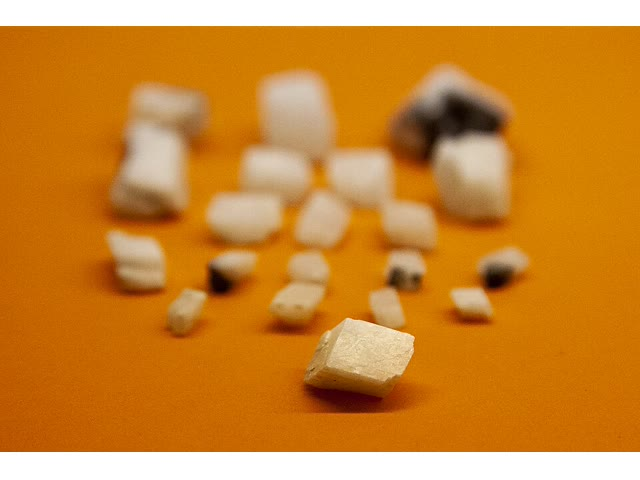
\includegraphics[width=\linewidth]{images/book3/b1-mineral-calcite-rhombs.jpg}

{\scriptsize معينات انشقاق الكالسيت. الصورة: Giovanna Canu وEva Santini، بترخيص CC BY 4.0 (Wikimedia Commons).}
\end{minipage}
\end{inthelab}

\begin{omfigure}
\setlength{\tabcolsep}{2pt}
\begin{tabular}{ccc}
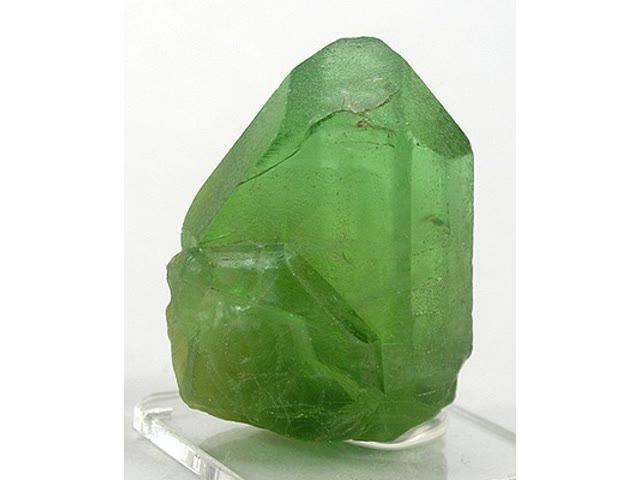
\includegraphics[width=0.31\linewidth]{images/book3/b1-mineral-olivine.jpg} &
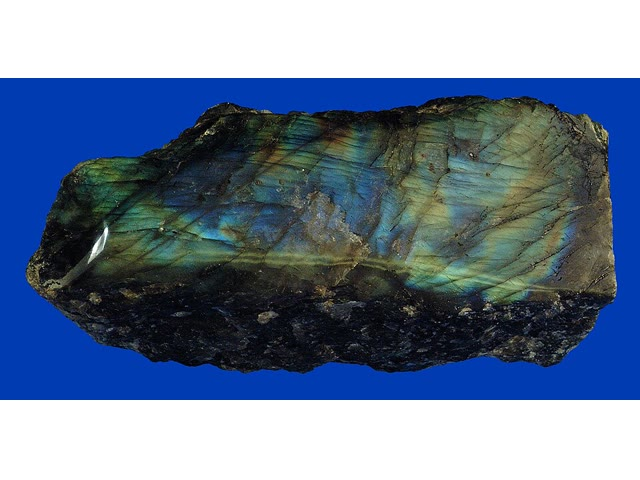
\includegraphics[width=0.31\linewidth]{images/book3/b1-mineral-plagioclase.jpg} &
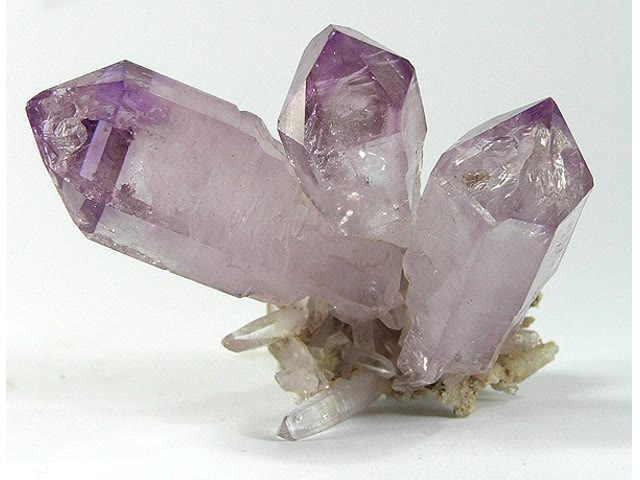
\includegraphics[width=0.31\linewidth]{images/book3/b1-mineral-quartz.jpg} \\
{\small (أ) \omterm{def:b1:rock-forming-minerals:groups}{الأوليفين}} & {\small (ب) \omterm{def:b1:rock-forming-minerals:groups}{البلاجيوكلاز} (لابرادوريت)} & {\small (ج) الكوارتز (أميثيست)} \\[4pt]
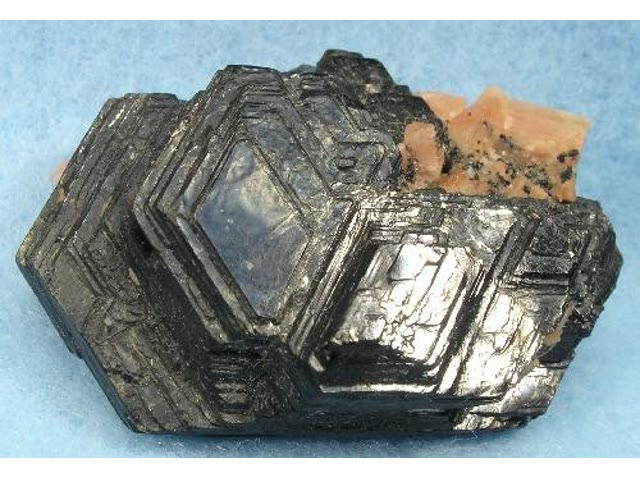
\includegraphics[width=0.31\linewidth]{images/book3/b1-mineral-biotite.jpg} &
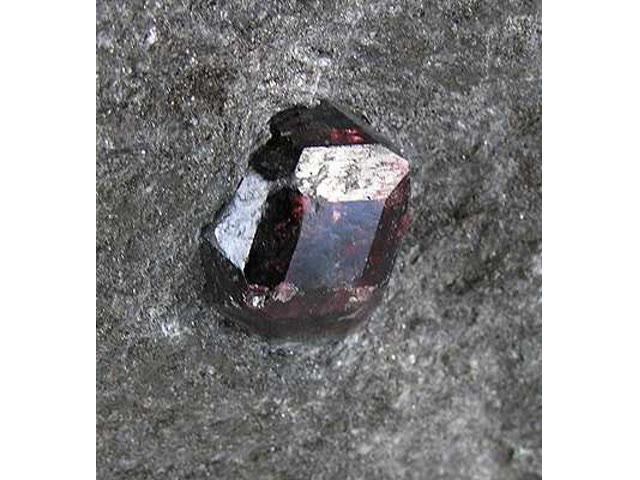
\includegraphics[width=0.31\linewidth]{images/book3/b1-mineral-garnet.jpg} &
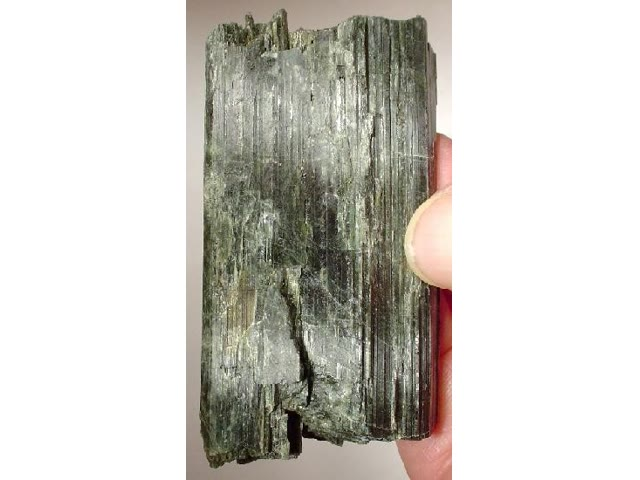
\includegraphics[width=0.31\linewidth]{images/book3/b1-mineral-hornblende.jpg} \\
{\small (د) البيوتيت على الأورثوكليز} & {\small (ه) \omterm{def:b1:rock-forming-minerals:groups}{الجارنيت} (ألماندين)} & {\small (و) هورنبلند} \\
\end{tabular}
\medskip
% ledger: commons:min-olivine, commons:min-plagioclase, commons:min-quartz, commons:min-biotite, commons:min-garnet, commons:min-hornblende

{\small ستة \omterm{def:b1:rock-forming-minerals:mineral}{معادن} مكوِّنة للصخور: (أ) بلورة \omterm{def:b1:rock-forming-minerals:groups}{أوليفين} جوهرية؛ (ب) شريحة مصقولة من \omterm{def:b1:rock-forming-minerals:groups}{البلاجيوكلاز} تُظهر لعب الألوان في اللابرادوريت؛ (ج) بلورات كوارتز، أعمدة سداسية الأضلاع برؤوس هرمية؛ (د) كتاب من رقائق البيوتيت على بلورة أورثوكليز؛ (ه) بلورة ألماندين من \omterm{def:b1:rock-forming-minerals:groups}{الجارنيت} في أرضيتها؛ (و) عمود من الهورنبلند. الصور (أ)، و(ج)--(و) ل Robert M.~Lavinsky، بترخيص CC BY-SA 3.0؛ و(ب) ل Twyla Baker، بترخيص CC0 (Wikimedia Commons).}
\end{omfigure}

\section{التمارين}

\begin{exercise}[$\star$]\label{exo:b1:rock-forming-minerals:1}
اذكر الصنف السيليكاتي لكل أنيون، وأعطِ عدد الرؤوس $s$ التي تتشاركها كل رباعية أوجه: \ce{SiO4^{4-}}، و\ce{Si2O7^{6-}}، و\ce{Si6O18^{12-}}، و\ce{Si2O5^{2-}}، و\ce{SiO2}. وإلى أيّ صنف يمكن أن ينتمي \ce{SiO3^{2-}}؟
\end{exercise}

\begin{exercise}[$\star$]\label{exo:b1:rock-forming-minerals:2}
مع الأوزان الذرية O \num{15.999}، وSi \num{28.085}، وMg \num{24.305}، وFe \qty{55.845}{g.mol^{-1}}، احسب الكتلتين المولَّيتين للفورستيريت والفايالايت، ثم حجميهما المولّيين من الكثافتين \num{3.275} و\qty{4.392}{g.cm^{-3}}.
% ledger: ciaaw:O, ciaaw:Si, ciaaw:Mg, ciaaw:Fe, hom:forsterite, hom:fayalite
\end{exercise}

\begin{exercise}[$\star$]\label{exo:b1:rock-forming-minerals:3}
في التناسق السداسي أنصاف الأقطار هي \ce{Mg^{2+}} \qty{0.72}{\angstrom}، و\ce{Fe^{2+}} \qty{0.78}{\angstrom}، و\ce{Ni^{2+}} \qty{0.69}{\angstrom}، و\ce{Mn^{2+}} \qty{0.83}{\angstrom}، و\ce{Ca^{2+}} \qty{1.00}{\angstrom}. احسب فرق كل منها عن نصف قطر \ce{Mg^{2+}} بالنسبة المئوية، وبيّن، بقواعد غولدشميت، أيّها يحل محل المغنيسيوم بحرية في \omterm{def:b1:rock-forming-minerals:groups}{الأوليفين}.
% ledger: shannon:radii, goldschmidt:size
\end{exercise}

\begin{exercise}[$\star$]\label{exo:b1:rock-forming-minerals:4}
للغرافيت والألماس كثافتان \num{2.16} و\qty{3.51}{g.cm^{-3}}؛ وللكالسيت والأراغونيت \num{2.71} و\qty{2.93}{g.cm^{-3}}. بكم في المئة ترتفع الكثافة في كل تغيير؟ وأي \omterm{def:b1:rock-forming-minerals:polymorph}{متعدد الأشكال} في كل زوج يتكوّن عند الضغط الأعلى؟
% ledger: webmineral:polymorphs, hom:calcite
\end{exercise}

\begin{exercise}[$\star\star$]\label{exo:b1:rock-forming-minerals:5}
اكتب \omterm{def:b1:rock-forming-minerals:formula}{الصيغة البنيوية} \omterm{def:b1:rock-forming-minerals:groups}{للبلاجيوكلاز} $\text{An}_{30}$ (\qty{30}{\percent} من المواقع الكبيرة يشغلها الكالسيوم)، وتحقق من أنها متعادلة.
\end{exercise}

\begin{exercise}[$\star\star$]\label{exo:b1:rock-forming-minerals:6}
في السلسلة المزدوجة، نصف الرباعيات يتشارك رأسين والنصف الآخر ثلاثة. عُدّ أكسجينات مجموعة متكررة من أربع رباعيات مباشرةً على اللوحة (و) من شكل الارتباط، وتحقّق من الصيغة \ce{Si4O11^{6-}} التي تعطيها \cref{prop:b1:rock-forming-minerals:si-o}.
\end{exercise}

\begin{exercise}[$\star\star$]\label{exo:b1:rock-forming-minerals:7}
أعد حساب تحليل \omterm{def:b1:rock-forming-minerals:groups}{أوليفين} على أربعة أكسجينات: \qty{40.20}{\percent} من \ce{SiO2}، و\qty{47.10}{\percent} من \ce{MgO}، و\qty{12.20}{\percent} من \ce{FeO}، و\qty{0.40}{\percent} من \ce{NiO} (الكتلة المولية ل\ce{NiO} هي \qty{74.692}{g.mol^{-1}}). أعطِ صيغته البنيوية، وتحقق منها، وأعطِ محتواها من الفورستيريت. ثم بيّن أنه يمكن استخراج محتوى الفورستيريت من نسبتي \ce{MgO} و\ce{FeO} وحدهما.
\end{exercise}

\begin{exercise}[$\star\star$]\label{exo:b1:rock-forming-minerals:8}
تحقّق من أن المسكوفيت \ce{KAl2(Si3Al)O10(OH)2} متعادل. فصفائحه من رباعيات الأوجه فيها ألومنيوم واحد مقابل ثلاثة سيليكونات: ما الشحنة التي يعطيها ذلك للصفيحة لكل صيغة وحدوية، وأيّ أيون يوازنها؟
\end{exercise}

\begin{exercise}[$\star\star$]\label{exo:b1:rock-forming-minerals:9}
باستعمال الحجمين المولّيين \num{42.96} و\qty{46.40}{cm^3.mol^{-1}} والكتلتين المولّيتين \num{140.691} و\qty{203.771}{g.mol^{-1}}: (أ) احسب كثافة $\text{Fo}_{50}$ بالخلط المثالي، وقارنها بمتوسط كثافتي الطرفين؛ (ب) أوجد محتوى الفورستيريت \omterm{def:b1:rock-forming-minerals:groups}{لأوليفين} كثافته \qty{3.600}{g.cm^{-3}}.
\end{exercise}

\begin{exercise}[$\star\star\star$]\label{exo:b1:rock-forming-minerals:10}
باستعمال تدوين \cref{prop:b1:rock-forming-minerals:ideal-mixing}، بيّن أن
\[
  \rho(x) - \bigl(x\rho_1 + (1 - x)\rho_2\bigr) =
  \frac{x(1 - x)(\rho_1 - \rho_2)(V_1 - V_2)}{V(x)} .
\]
ويُستنتج أن كثافة \omterm{def:b1:rock-forming-minerals:groups}{الأوليفين} تقع أعلى من الخط المستقيم بين \omterm{def:b1:rock-forming-minerals:solid-solution}{الأطراف}، واحسب الفجوة عند $\text{Fo}_{50}$.
\end{exercise}

\begin{exercise}[$\star\star\star$]\label{exo:b1:rock-forming-minerals:11}
يعطي \omterm{def:b1:rock-forming-minerals:groups}{بلاجيوكلاز} من جابرو \qty{54.10}{\percent} من \ce{SiO2}، و\qty{28.90}{\percent} من \ce{Al2O3}، و\qty{11.20}{\percent} من \ce{CaO}، و\qty{5.10}{\percent} من \ce{Na2O}، و\qty{0.30}{\percent} من \ce{K2O} (الكتل المولية \num{60.083}، و\num{101.961}، و\num{56.077}، و\num{61.979}، و\qty{94.195}{g.mol^{-1}}). أعد حسابه على ثمانية أكسجينات؛ وتحقّق من أن الرباعيات (Si + Al) تحوي 4 ذرات، والموقع الكبير (Ca + Na + K) ذرة واحدة؛ وتحقّق من \omterm{def:b1:rock-forming-minerals:substitution}{الإحلال المقترن} بمقارنة $\mathrm{Al} - 1$ بالكالسيوم؛ وأعطِ محتوى الأنورثيت $100\,\mathrm{Ca}/(\mathrm{Ca} +
\mathrm{Na} + \mathrm{K})$.
\end{exercise}

\begin{exercise}[$\star\star\star$]\label{exo:b1:rock-forming-minerals:12}
لا يستطيع المسبار أن يميّز \ce{Fe^{2+}} من \ce{Fe^{3+}}، فيُبلّغ عن كل الحديد على صورة \ce{FeO}. (أ) بيّن أن المغنتيت النقي \ce{Fe3O4}، إذا حُلّل بهذه الطريقة، يبلغ مجموعه \qty{93.09}{\percent}. (ب) أعد حساب هذا التحليل على أربعة أكسجينات، وبيّن لماذا تكون النتيجة مستحيلة \omterm{def:b1:rock-forming-minerals:mineral}{لمعدن} فيه ثلاثة كاتيونات لكل أربعة أكسجينات. (ج) أعد الحساب على ثلاثة كاتيونات بدلًا من ذلك، وأوجد عدد \ce{Fe^{2+}} و\ce{Fe^{3+}} بطلب أن تكون الصيغة متعادلة. (د) أعد التعبير عن التحليل على صورة \ce{FeO} و\ce{Fe2O3}، وأعطِ المجموع الجديد.
\end{exercise}

\section{مسألة: أوليفين من بازلت}

\begin{problem}[{مسألة نهاية الأسبوع --- إعادة حساب تحليل بالمسبار لأوليفين، وكتابة صيغته والتحقق منها، وإيجاد تركيبه وكثافته وكتلته في متر مكعب من البازلت}]
\label{pb:b1:rock-forming-minerals:1}
% invented analysis: figdata/bachelor-1/solid_solution.py (OLIVINE_WT); values: calc/ch07.py
% ledger: ciaaw:O, ciaaw:Si, ciaaw:Mg, ciaaw:Fe, ciaaw:Mn, ciaaw:Ni, ciaaw:Ca, hom:forsterite, hom:fayalite, shannon:radii
البلورات الخضراء لبازلت هي \omterm{def:b1:rock-forming-minerals:groups}{الأوليفين}. ويعطي تحليل بالمسبار لإحداها، بالنسبة المئوية الوزنية للأكاسيد:
\begin{center}
\small
\begin{tabular}{lcccccc}
\hline
الأكسيد & \ce{SiO2} & \ce{FeO} & \ce{MnO} & \ce{MgO} & \ce{NiO} & \ce{CaO} \\
نسبة الوزن \% & 39.50 & 16.53 & 0.23 & 43.32 & 0.20 & 0.22 \\
\hline
\end{tabular}
\end{center}
الأوزان الذرية هي O \num{15.999}، وSi \num{28.085}، وFe \num{55.845}، وMn \num{54.938}، وMg \num{24.305}، وNi \num{58.693}، وCa \qty{40.078}{g.mol^{-1}}. وللفورستيريت كثافة \qty{3.275}{g.cm^{-3}}، وللفايالايت \qty{4.392}{g.cm^{-3}}.

\medskip
\noindent\textbf{الجزء الأول --- من الأكاسيد إلى الكاتيونات.}
\begin{enumerate}
  \item احسب الكتل المولية للأكاسيد الستة.
  \item احسب مجموع التحليل. ماذا كان سيوحي به مجموع قدره \qty{97}{\percent}؟
  \item احسب عدد مولات كل أكسيد في \qty{100}{g} من \omterm{def:b1:rock-forming-minerals:groups}{الأوليفين}.
  \item احسب مولات الأكسجين التي تحويها، ومجموعها.
  \item احسب مولات كل كاتيون.
  \item احسب المعامل الذي يجعل الأكسجينات أربعة.
  \item أعطِ عدد ذرات كل عنصر لكل أربعة أكسجينات، إلى ثلاث منازل عشرية.
\end{enumerate}

\medskip
\noindent\textbf{الجزء الثاني --- \omterm{def:b1:rock-forming-minerals:formula}{الصيغة البنيوية}.}
\begin{enumerate}[resume]
  \item \omterm{def:b1:rock-forming-minerals:groups}{للأوليفين} موقع رباعي واحد ومركزان ثمانيان لكل أربعة أكسجينات. احسب مجموع الكاتيونات غير السيليكون، وقارن مجموعي المواقع بالصيغة المثالية.
  \item اكتب \omterm{def:b1:rock-forming-minerals:formula}{الصيغة البنيوية} \omterm{def:b1:rock-forming-minerals:groups}{للأوليفين}.
  \item تحقّق من أن الصيغة متعادلة، وفسّر لماذا لم يكن لهذا التحقق، بخلاف ما في السؤال 8، أن يفشل.
  \item باستعمال أنصاف الأقطار الأيونية (\ce{Mg^{2+}} \qty{0.72}{\angstrom}، و\ce{Fe^{2+}} \qty{0.78}{\angstrom}، و\ce{Ni^{2+}} \qty{0.69}{\angstrom}، و\ce{Mn^{2+}} \qty{0.83}{\angstrom}، و\ce{Ca^{2+}} \qty{1.00}{\angstrom}، كلها في التناسق السداسي)، فسّر لماذا يكون النيكل شائعًا في \omterm{def:b1:rock-forming-minerals:groups}{الأوليفين} والكالسيوم نادرًا.
  \item يُبلّغ المسبار عن كل الحديد على صورة \ce{FeO}. فسّر لماذا يبيّن مجموع الكاتيونات الموجود في السؤال 7 أن \omterm{def:b1:rock-forming-minerals:groups}{الأوليفين} لا يحوي \ce{Fe^{3+}} يُعتدّ به.
\end{enumerate}

\medskip
\noindent\textbf{الجزء الثالث --- التركيب.}
\begin{enumerate}[resume]
  \item احسب محتوى الفورستيريت $\mathrm{Fo} = 100\,\mathrm{Mg}/(\mathrm{Mg} +
        \mathrm{Fe})$، إلى منزلة عشرية واحدة.
  \item ما \omterm{def:b1:rock-forming-minerals:formula}{رقم المغنيسيوم} \omterm{def:b1:rock-forming-minerals:groups}{للأوليفين}؟ ولماذا يساوي محتوى الفورستيريت هنا؟
  \item اكتب \omterm{def:b1:rock-forming-minerals:groups}{الأوليفين} محلولًا صلبًا ثنائيًا $\mathrm{Fo}_x\mathrm{Fa}_{1-x}$، متجاهلًا Mn وNi وCa، وأعطِ نسبة مواقعه الثمانية التي يشغلها الحديد.
  \item بيّن أنه يمكن حساب محتوى الفورستيريت من نسبتي \ce{MgO} و\ce{FeO} وحدهما، دون معامل السؤال 6، واحسبه.
  \item \omterm{def:b1:rock-forming-minerals:groups}{أوليفين} نما لاحقًا في الحمم نفسها فيه \qty{40.5}{\percent} من \ce{MgO} و\qty{20.0}{\percent} من \ce{FeO}. احسب محتواه من الفورستيريت. أيّ الأوليفينين أغنى بالحديد؟
\end{enumerate}

\medskip
\noindent\textbf{الجزء الرابع --- الكثافة والكتلة.}
\begin{enumerate}[resume]
  \item احسب الكتل المولية والحجوم المولية للفورستيريت والفايالايت (الحجوم المولية إلى منزلتين عشريتين).
  \item باعتبار \omterm{def:b1:rock-forming-minerals:groups}{الأوليفين} الثنائي $\mathrm{Fo}_x\mathrm{Fa}_{1-x}$ في السؤال 15، مع تقريب $x$ إلى ثلاث منازل عشرية، احسب كتلته المولية وحجمه المولي بالخلط المثالي.
  \item استنتج كثافته، إلى ثلاث منازل عشرية.
  \item قارنها بالاستكمال الخطي بين كثافتي \omterm{def:b1:rock-forming-minerals:solid-solution}{الأطراف}.
  \item يحوي البازلت \qty{12}{\percent} من \omterm{def:b1:rock-forming-minerals:groups}{الأوليفين} بالحجم. ما كتلة \omterm{def:b1:rock-forming-minerals:groups}{الأوليفين} التي يحويها متر مكعب من البازلت؟
  \item كثافة البازلت \qty{2.95}{g.cm^{-3}}. ما نسبة \omterm{def:b1:rock-forming-minerals:groups}{الأوليفين} بالكتلة؟
  \item ما محتوى الفورستيريت \omterm{def:b1:rock-forming-minerals:groups}{للأوليفين}، مقرّبًا إلى أقرب نسبة مئوية كاملة؟
\end{enumerate}
\end{problem}
